\chapter{Design requirements}

In this chapter the requirement for the TID sensor will be presented.

Sensor is designed to be flown on-board of PW-Sat2 satellite. Therefore it should be designed for its particular requirements. In addition, it should be designed having in mind active space standard and launcher requirements.


\section{PW-Sat2 mission}
	Presented sensor is scheduled to be launched on PW-Sat2 satellite \cite{PW-Sat2URL}. Therefore it should be designed especially for this particular type of mission. In this section PW-Sat2 mission will be presented. On fig. \ref{PW-Sat_render_01} exploded render is presented.
	
	\begin{figure}[h]
		\centering
		\includegraphics[width=0.5\paperwidth]{img/PW-Sat2_render_01.png}
		\caption{PW-Sat2 render (by M. Świetlik)}
		\label{PW-Sat_render_01}
	\end{figure}

	PW-Sat2 is scheduled to be launched on Falon9 rocket from SpaceX company in Q4 2017.
	
	\begin{figure}[H]
		\centering
		\includegraphics[width=0.3\paperwidth]{img/Falcon9.jpg}
		\caption{Falcon9 rocket. Source: \url{www.spacex.com}}
		\label{PW-Sat_render_01}
	\end{figure}
	
	
\subsection{Primary mission}
	Primary mission of PW-Sat2 is to test deorbiting sail. Its purpose is to increase atmospheric drag and shorten satellite life. This method of deorbitation could be easy way to reduce space debris on LEO. Render of PW-Sat2 with opened sail is on \ref{PW-Sat_render_sail}.
	
	\begin{figure}[H]
		\centering
		\includegraphics[width=0.7\paperwidth]{img/PW-Sat2_render_02.png}
		\caption{PW-Sat2 with opened sail (by M. Świetlik)}
		\label{PW-Sat_render_sail}
	\end{figure}
	
	More information can be found in \cite{DDC_article}.
	
\subsection{Lifetime}
	Due to its primary mission PW-Sat2 mission is planned to be 40 days long. After this time deorbit sail will open, possibly causing lack of communication with satellite. Therefore sensor should be able to measure dose absorbed during 40 days on orbit.
	
\subsection{Orbit}
	PW-Sat2 in planned to be launched to sun-synchronous circular orbit of attitude $575~km$, with LTAN of $10:30$ \cite{PWSAT_MA_CDR}.
	

\subsection{Radiation analysis}
	Simulations in SPENVIS \cite{SPENVIS_URL} were performed to determine TID accumulated during PW-Sat2 mission. On fig \ref{TIDvsSheilding} dose as a function of shielding thickness was plotted.

	\begin{figure}[H]
		\centering
		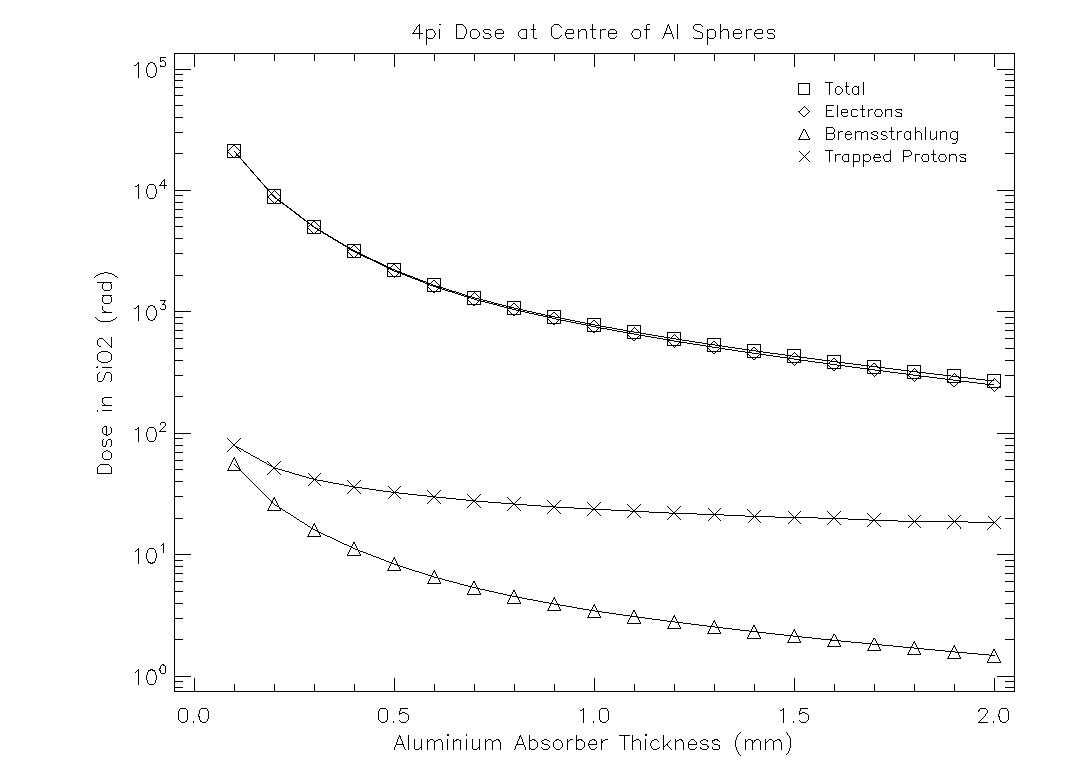
\includegraphics[width=0.7\paperwidth]{img/dose.eps}
		\caption{TID vs shielding}
		\label{TIDvsSheilding}
	\end{figure}

	Shielding of PW-Sat2 is about $1~mm$ thick (aluminium sides as well as aluminium base for solar cells - \ref{PW-Sat_render_01}). Therefore predicted dose during PW-Sat2 mission is about $1$~kRad.


\section{Sensor requirements}
	In this section sensor requirements are presented.

\subsection{Range}
	Total range of the sensor should be more than predicted dose ($>~1$~kRad). With $300\%$ reserve: designed sensor should have range of more than $3$~kRad.
	
\subsection{Accuracy \& resolution}
	Sensor should be able to detect low radiation doses. Its resolution should be lower than $0.1$~kRad, with accuracy of less than $0.5$~kRad.


\section{Electrical requirements}
	
\subsection{Electronics stack}
\subsection{Power}
\subsection{Data interface}
\subsection{Radiation immunity}
\subsection{Reliability of components}

\section{Mechanical requirements}
\subsection{PCB stack \& PCB restrictions}
\subsection{Space available}
\subsection{Vibration}
\subsection{Operation temperature}
\subsection{Thermal cycles}

\section{Applicable standards}